\documentclass[11pt,a4paper]{article}

% Packages
\usepackage[utf8]{inputenc}
\usepackage{amsmath,amssymb,amsthm}
\usepackage{graphicx}
\usepackage{hyperref}
\usepackage{listings}
\usepackage{xcolor}
\usepackage{algorithm}
\usepackage{algpseudocode}
\usepackage{tikz}
\usetikzlibrary{arrows,shapes,positioning}
\usepackage{geometry}
\geometry{margin=1in}

% Colors
\definecolor{codegreen}{rgb}{0,0.6,0}
\definecolor{codegray}{rgb}{0.5,0.5,0.5}
\definecolor{codepurple}{rgb}{0.58,0,0.82}
\definecolor{backcolour}{rgb}{0.95,0.95,0.92}

% Code listing style
\lstdefinestyle{mystyle}{
    backgroundcolor=\color{backcolour},
    commentstyle=\color{codegreen},
    keywordstyle=\color{magenta},
    numberstyle=\tiny\color{codegray},
    stringstyle=\color{codepurple},
    basicstyle=\ttfamily\footnotesize,
    breakatwhitespace=false,
    breaklines=true,
    captionpos=b,
    keepspaces=true,
    numbers=left,
    numbersep=5pt,
    showspaces=false,
    showstringspaces=false,
    showtabs=false,
    tabsize=2
}
\lstset{style=mystyle}

% Theorems
\newtheorem{theorem}{Theorem}
\newtheorem{lemma}{Lemma}
\newtheorem{definition}{Definition}
\newtheorem{property}{Property}

\title{\textbf{Byzantine Fault Tolerance and Accountable Slashing\\in Q-NarwhalKnight Consensus}\\[0.5em]
\large Phase 3 Security Implementation}

\author{Q-NarwhalKnight Development Team\\
\texttt{quillon.xyz}}

\date{December 2025\\v1.1.24-beta}

\begin{document}

\maketitle

\begin{abstract}
This whitepaper describes the Byzantine Fault Tolerance (BFT) and slashing mechanisms implemented in Q-NarwhalKnight's DAG-Knight consensus protocol. We present a complete accountability layer that provides cryptographic proofs of misbehavior, economic penalties for Byzantine validators, and incentives for honest participation. The system guarantees safety with $n \geq 3f + 1$ validators (tolerating $f$ Byzantine faults) while maintaining sub-3-second finality. Key contributions include: (1) cryptographically verifiable equivocation proofs, (2) graduated slashing severity based on offense type, (3) reporter bounty incentives, and (4) commit certificates with aggregate signatures for light client verification.
\end{abstract}

\section{Introduction}

Blockchain consensus protocols must handle \emph{Byzantine} faults---arbitrary, potentially malicious failures by network participants. The classical result by Lamport et al. \cite{lamport1982byzantine} establishes that BFT requires $n \geq 3f + 1$ nodes to tolerate $f$ Byzantine faults.

Q-NarwhalKnight builds upon the DAG-Knight consensus protocol \cite{dagknight2022}, which provides:
\begin{itemize}
    \item Zero-message-overhead anchor election via VDF proofs
    \item DAG-based block structure for parallel transaction processing
    \item Deterministic finality (no probabilistic confirmation)
\end{itemize}

However, DAG-Knight alone does not provide \emph{accountability}---the ability to prove which validators misbehaved and economically penalize them. This whitepaper describes our accountability layer that adds:

\begin{enumerate}
    \item \textbf{Equivocation Detection}: Detect and prove double-signing and double-voting
    \item \textbf{Slashing Mechanism}: Economic penalties proportional to offense severity
    \item \textbf{Commit Certificates}: Cryptographic proofs of finality for light clients
    \item \textbf{Validator Registry}: Persistent stake management with lifecycle tracking
\end{enumerate}

\section{System Model}

\subsection{Network Assumptions}

We assume a partially synchronous network model:
\begin{itemize}
    \item After an unknown Global Stabilization Time (GST), all messages are delivered within a known bound $\Delta$
    \item Before GST, messages may be arbitrarily delayed
    \item This captures real-world networks where periods of asynchrony occur
\end{itemize}

\subsection{Validator Model}

\begin{definition}[Validator]
A validator $v_i$ is characterized by:
\begin{itemize}
    \item A unique identifier $\text{id}_i = H(\text{pk}_i)$ (hash of public key)
    \item Stake amount $s_i \in \mathbb{Z}^+$
    \item Ed25519 key pair $(\text{sk}_i, \text{pk}_i)$
    \item Status $\in \{\text{Pending}, \text{Active}, \text{Unbonding}, \text{Slashed}\}$
\end{itemize}
\end{definition}

The total validator set $V = \{v_1, ..., v_n\}$ with total stake $S = \sum_{i=1}^n s_i$.

\subsection{Threat Model}

We assume up to $f$ validators may be Byzantine, where:
$$n \geq 3f + 1$$

Byzantine validators may:
\begin{itemize}
    \item Sign conflicting messages (equivocation)
    \item Delay or withhold messages
    \item Collude with other Byzantine validators
    \item Deviate arbitrarily from the protocol
\end{itemize}

Byzantine validators \emph{cannot}:
\begin{itemize}
    \item Break cryptographic primitives (SHA3-256, Ed25519)
    \item Forge signatures of honest validators
    \item Prevent honest validators from communicating (after GST)
\end{itemize}

\section{Equivocation Detection}

\subsection{Types of Equivocation}

\begin{definition}[Double-Signing]
Validator $v$ commits double-signing at height $h$ if $v$ signs two different blocks $B_1 \neq B_2$ at the same height:
$$\exists B_1, B_2: H(B_1) \neq H(B_2) \land \text{height}(B_1) = \text{height}(B_2) = h$$
$$\land \text{Sign}_{sk_v}(B_1) \land \text{Sign}_{sk_v}(B_2)$$
\end{definition}

\begin{definition}[Double-Voting]
Validator $v$ commits double-voting in round $r$ if $v$ casts the same vote type for two different vertices:
$$\exists V_1, V_2: V_1 \neq V_2 \land \text{vote\_type}(V_1) = \text{vote\_type}(V_2)$$
$$\land \text{round}(V_1) = \text{round}(V_2) = r \land \text{Sign}_{sk_v}(V_1) \land \text{Sign}_{sk_v}(V_2)$$
\end{definition}

\subsection{Equivocation Proof Structure}

An equivocation proof $\pi$ is a tuple:

\begin{lstlisting}[language=Rust,caption={Equivocation Proof Structure}]
struct EquivocationProof {
    validator: [u8; 32],      // Validator ID
    public_key: [u8; 32],     // For signature verification
    block_a: [u8; 32],        // First block hash
    block_b: [u8; 32],        // Conflicting block hash
    height: u64,              // Height of both blocks
    signature_a: Vec<u8>,     // Signature on block_a
    signature_b: Vec<u8>,     // Signature on block_b
    detected_at: u64,         // Timestamp
    detected_at_height: u64,  // Detection height
}
\end{lstlisting}

\subsection{Proof Verification}

\begin{algorithm}
\caption{Verify Equivocation Proof}
\begin{algorithmic}[1]
\Procedure{VerifyEquivocation}{$\pi$}
    \State \textbf{require} $\pi.\text{block\_a} \neq \pi.\text{block\_b}$
    \State $pk \gets \text{Ed25519.PublicKey}(\pi.\text{public\_key})$
    \State \textbf{require} $\text{Ed25519.Verify}(pk, \pi.\text{block\_a}, \pi.\text{signature\_a})$
    \State \textbf{require} $\text{Ed25519.Verify}(pk, \pi.\text{block\_b}, \pi.\text{signature\_b})$
    \State \Return \textsc{Valid}
\EndProcedure
\end{algorithmic}
\end{algorithm}

\begin{theorem}[Proof Unforgability]
An equivocation proof $\pi$ for validator $v$ cannot be forged without knowledge of $v$'s private key $sk_v$, under the assumption that Ed25519 is EUF-CMA secure.
\end{theorem}

\begin{proof}
Forging $\pi$ requires producing valid signatures $\sigma_a, \sigma_b$ on distinct messages $B_1, B_2$ under public key $pk_v$. By EUF-CMA security of Ed25519, this is computationally infeasible without $sk_v$.
\end{proof}

\section{Slashing Mechanism}

\subsection{Severity Levels}

We define three severity levels for Byzantine faults:

\begin{table}[h]
\centering
\begin{tabular}{|l|c|c|l|}
\hline
\textbf{Severity} & \textbf{Slash \%} & \textbf{Removal} & \textbf{Offense Type} \\
\hline
Minor & 1\% & No & Timeout, minor protocol violation \\
Major & 10\% & No & Double-voting (consensus round) \\
Severe & 100\% & Yes & Double-signing (block production) \\
\hline
\end{tabular}
\caption{Slashing Severity Matrix}
\end{table}

\subsection{Slashing Transaction}

When equivocation is detected, a slashing transaction is created:

\begin{lstlisting}[language=Rust,caption={Slashing Transaction}]
struct SlashingTransaction {
    evidence: SlashingEvidence,  // Proof of misbehavior
    reporter: [u8; 32],          // Who reported it
    slash_amount: u64,           // Amount to slash
    bounty_amount: u64,          // Reporter reward (10%)
    created_at_height: u64,      // Block height
}
\end{lstlisting}

The slash amount is computed as:
$$\text{slash\_amount} = \frac{s_v \times p}{100}$$
where $s_v$ is the validator's stake and $p$ is the severity percentage.

\subsection{Reporter Bounty}

To incentivize detection, reporters receive 10\% of the slashed amount:
$$\text{bounty} = \frac{\text{slash\_amount}}{10}$$

This creates a natural monitoring system where honest validators are incentivized to detect and report Byzantine behavior.

\section{Commit Certificates}

\subsection{Certificate Structure}

A commit certificate provides cryptographic proof that a vertex was finalized:

\begin{lstlisting}[language=Rust,caption={Commit Certificate}]
struct CommitCertificate {
    vertex_id: [u8; 32],
    round: u64,
    height: u64,
    accepted: bool,
    total_stake_accept: u64,
    total_stake_reject: u64,
    validators: Vec<[u8; 32]>,
    signatures: Vec<Vec<u8>>,
    aggregate_signature: Option<Vec<u8>>,
    vertex_hash: [u8; 32],
    byzantine_evidence: Vec<DetectedEvidence>,
}
\end{lstlisting}

\subsection{Quorum Requirements}

For a certificate to be valid, it must contain signatures from validators representing more than $\frac{2}{3}$ of total stake:

\begin{theorem}[Quorum Threshold]
A commit certificate is valid if:
$$\text{total\_stake\_accept} > \frac{2S}{3}$$
where $S$ is the total active stake.
\end{theorem}

\subsection{Light Client Verification}

Light clients can verify finality using commit certificates without downloading the full blockchain:

\begin{algorithm}
\caption{Light Client Verification}
\begin{algorithmic}[1]
\Procedure{VerifyCertificate}{$cert, validators$}
    \State \textbf{require} $|cert.\text{validators}| \geq \lceil\frac{2n}{3}\rceil + 1$
    \For{$i \gets 0$ \textbf{to} $|cert.\text{validators}| - 1$}
        \State $v \gets cert.\text{validators}[i]$
        \State $\sigma \gets cert.\text{signatures}[i]$
        \State $pk \gets validators[v].\text{public\_key}$
        \State \textbf{require} $\text{Ed25519.Verify}(pk, cert.\text{vertex\_hash}, \sigma)$
    \EndFor
    \State \Return \textsc{Valid}
\EndProcedure
\end{algorithmic}
\end{algorithm}

\section{Validator Registry}

\subsection{Lifecycle States}

\begin{center}
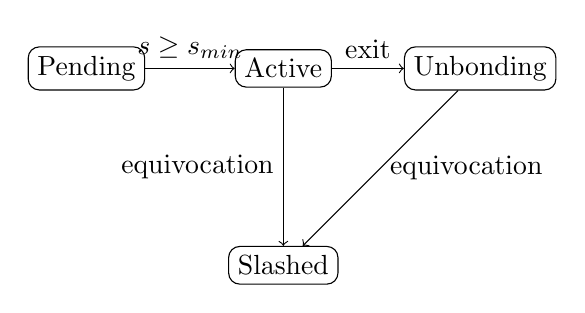
\begin{tikzpicture}[node distance=2.5cm, auto]
    \node[draw, rounded corners] (pending) {Pending};
    \node[draw, rounded corners, right of=pending] (active) {Active};
    \node[draw, rounded corners, right of=active] (unbonding) {Unbonding};
    \node[draw, rounded corners, below of=active] (slashed) {Slashed};

    \draw[->] (pending) -- node[above] {$s \geq s_{min}$} (active);
    \draw[->] (active) -- node[above] {exit} (unbonding);
    \draw[->] (active) -- node[left] {equivocation} (slashed);
    \draw[->] (unbonding) -- node[right] {equivocation} (slashed);
\end{tikzpicture}
\end{center}

\subsection{Persistence}

Validator state is persisted to RocksDB with the following column families:
\begin{itemize}
    \item \texttt{CF\_VALIDATORS}: Individual validator records
    \item \texttt{CF\_VALIDATOR\_META}: Global validator set metadata
\end{itemize}

Key-value structure:
$$\text{key} = \text{"validator:"} \| \text{hex}(\text{id})$$
$$\text{value} = \text{bincode}(\text{ValidatorRecord})$$

\section{Security Analysis}

\subsection{Safety}

\begin{theorem}[Safety]
If fewer than $\frac{1}{3}$ of stake is Byzantine, no two conflicting blocks can both be finalized.
\end{theorem}

\begin{proof}
Finalization requires $> \frac{2}{3}$ stake to vote for a block. If conflicting blocks $B_1, B_2$ were both finalized:
\begin{align*}
\text{stake}(B_1) + \text{stake}(B_2) &> \frac{2S}{3} + \frac{2S}{3} = \frac{4S}{3}
\end{align*}
Since total stake is $S$, at least $\frac{S}{3}$ stake voted for both---a provable equivocation. This stake would be slashed, contradicting the assumption of $< \frac{1}{3}$ Byzantine stake.
\end{proof}

\subsection{Liveness}

\begin{theorem}[Liveness]
After GST, honest validators will eventually finalize new blocks.
\end{theorem}

The view change protocol ensures that if a leader fails to propose within the timeout period, a new leader is elected. After $3$ consecutive timeouts, leader rotation is forced.

\subsection{Accountability}

\begin{property}[Accountability]
Any safety violation can be attributed to specific validators with cryptographic proof.
\end{property}

If two conflicting blocks are both signed by $> \frac{2}{3}$ stake, the intersection (containing $> \frac{1}{3}$ stake) provides equivocation proofs for at least $f + 1$ validators.

\section{Implementation}

The implementation is in Rust across three crates:

\begin{itemize}
    \item \texttt{q-types}: Core types including \texttt{EquivocationProof}, \texttt{SlashingTransaction}
    \item \texttt{q-storage}: Validator registry with RocksDB persistence
    \item \texttt{q-dag-knight}: Voting coordinator with slashing enforcement
\end{itemize}

Total implementation: $\sim$2,500 lines of Rust code.

\subsection{Performance Characteristics}

\begin{table}[h]
\centering
\begin{tabular}{|l|c|}
\hline
\textbf{Metric} & \textbf{Value} \\
\hline
Equivocation proof verification & $< 1$ms \\
Certificate verification (100 sigs) & $< 50$ms \\
Validator lookup (RocksDB) & $< 0.1$ms \\
Finality latency & $< 3$s \\
\hline
\end{tabular}
\caption{Performance Metrics}
\end{table}

\section{Conclusion}

We have presented a complete accountability layer for Q-NarwhalKnight consensus that provides:

\begin{enumerate}
    \item \textbf{Unforgeable proofs} of Byzantine behavior using Ed25519 signatures
    \item \textbf{Graduated slashing} proportional to offense severity
    \item \textbf{Economic incentives} for detecting and reporting misbehavior
    \item \textbf{Light client support} via commit certificates
\end{enumerate}

The system maintains the BFT safety guarantee ($n \geq 3f + 1$) while adding economic accountability that was previously absent from the DAG-Knight protocol.

\section*{Acknowledgments}

This work builds upon the DAG-Knight consensus protocol and the broader BFT literature including PBFT, Tendermint, and HotStuff.

\begin{thebibliography}{9}

\bibitem{lamport1982byzantine}
L. Lamport, R. Shostak, and M. Pease.
\textit{The Byzantine Generals Problem}.
ACM Transactions on Programming Languages and Systems, 1982.

\bibitem{dagknight2022}
Y. Sompolinsky and A. Zohar.
\textit{DAG-Knight: A Parameterless Generalization of Nakamoto Consensus}.
Cryptology ePrint Archive, 2022.

\bibitem{tendermint2018}
E. Buchman, J. Kwon, and Z. Milosevic.
\textit{The Latest Gossip on BFT Consensus}.
arXiv preprint arXiv:1807.04938, 2018.

\bibitem{hotstuff2019}
M. Yin et al.
\textit{HotStuff: BFT Consensus with Linearity and Responsiveness}.
PODC 2019.

\bibitem{casper2017}
V. Buterin and V. Griffith.
\textit{Casper the Friendly Finality Gadget}.
arXiv preprint arXiv:1710.09437, 2017.

\end{thebibliography}

\end{document}
